\section{実験結果}

表\ref{tbl:実験結果}に各試験片の四点曲げ試験の結果及び寸法を示す.

\begin{table}[htbp]
    \centering
    \caption{Four-point bending test results and dimensions of each specimen.}
    \label{tbl:実験結果}
    \scalebox{0.7}{
    \begin{tabular}{|c|c|c|cc|}
    \hline
                   &                &                   & \multicolumn{2}{c|}{寸法}                     \\ \hline
                   & 破断時の荷重{[}kN{]} & 破断時のストローク{[}mm{]} & \multicolumn{1}{c|}{厚み{[}mm{]}} & 幅{[}mm{]} \\ \hline
    1(傷なし)         & 0.0572         & 0.444             & \multicolumn{1}{c|}{1.25}       & 25.90     \\ \hline
    2(傷なし)         & 0.0844         & 0.617             & \multicolumn{1}{c|}{1.25}       & 25.90     \\ \hline
    3(傷なし)         & 0.0571         & 0.427             & \multicolumn{1}{c|}{1.20}       & 25.90     \\ \hline
    4(傷なし)         & 0.0703         & 0.500             & \multicolumn{1}{c|}{1.25}       & 25.95     \\ \hline
    5(傷なし)\_ひずみゲージ & 0.0553         & 0.411             & \multicolumn{1}{c|}{1.30}       & 26.00     \\ \hline
    1(傷あり)         & 0.0307         & 0.253             & \multicolumn{1}{c|}{1.25}       & 26.10     \\ \hline
    2(傷あり)         & 0.0392         & 0.300             & \multicolumn{1}{c|}{1.25}       & 25.80     \\ \hline
    3(傷あり)         & 0.0425         & 0.333             & \multicolumn{1}{c|}{1.20}       & 25.85     \\ \hline
    4(傷あり)         & 0.0374         & 0.322             & \multicolumn{1}{c|}{1.25}       & 25.85     \\ \hline
    5(傷あり)         & 0.0423         & 0.331             & \multicolumn{1}{c|}{1.25}       & 25.90     \\ \hline
    \end{tabular}
    }
\end{table}

ひずみゲージにより得られた荷重-ひずみ線図を図\ref{fig:荷重ひずみ線図}に,応力-ひずみ線図を図\ref{fig:応力ひずみ線図}に示す.
\begin{figure}[htbp]
    \centering %中央揃え
    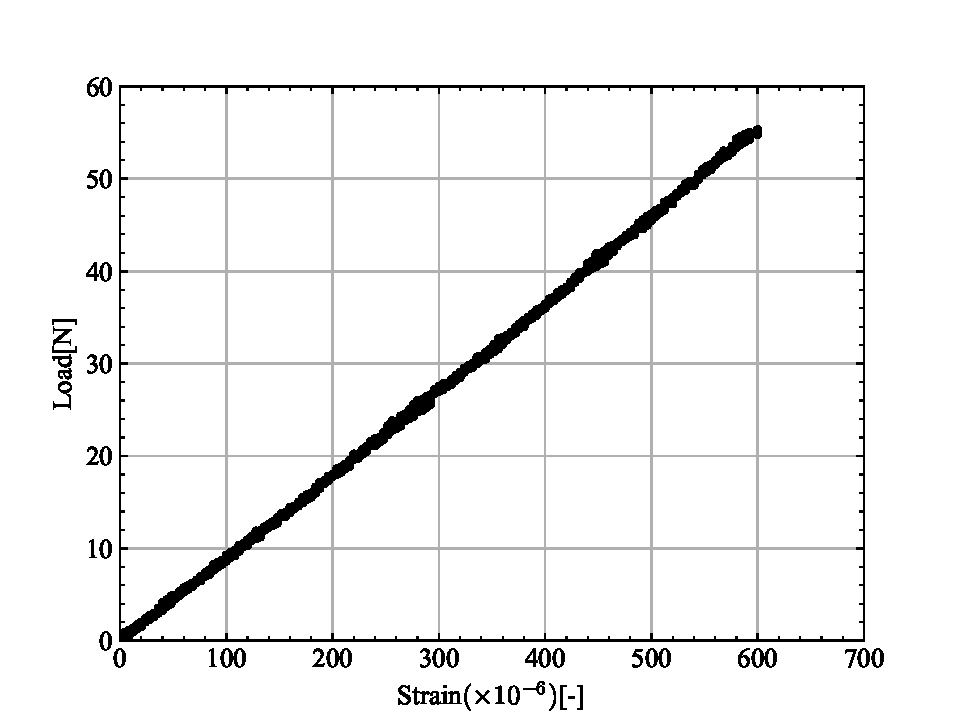
\includegraphics[width=100truemm,clip]{fig/fig_LoadStrain.pdf}
    \caption{Load strain diagram.}
    \label{fig:荷重ひずみ線図}
\end{figure}
\begin{figure}[htbp]
    \centering %中央揃え
    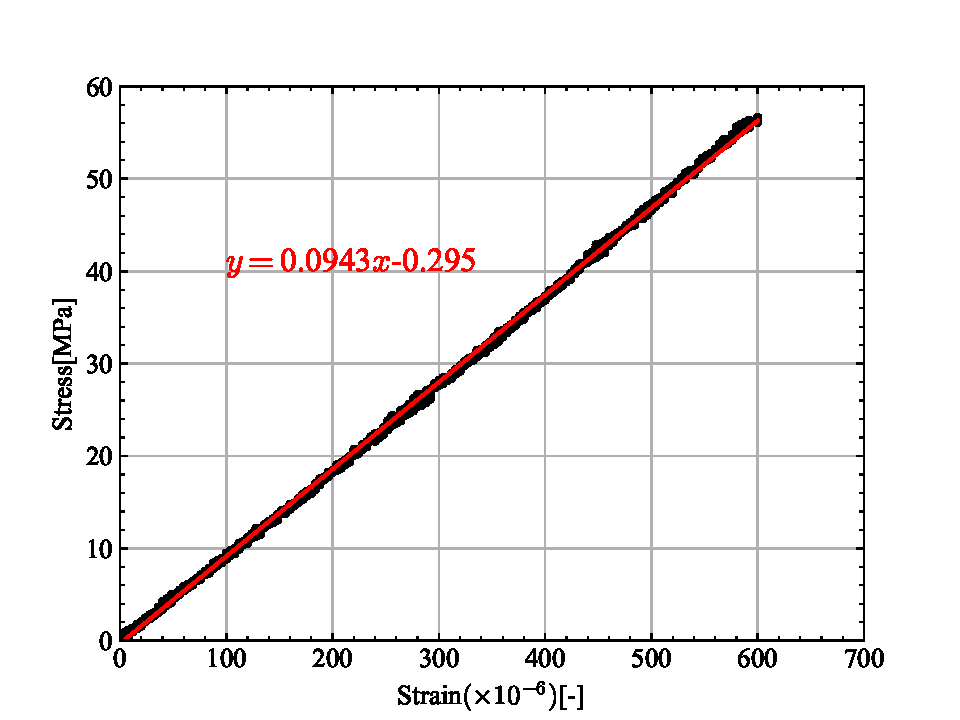
\includegraphics[width=100truemm,clip]{fig/fig_StressStrain.pdf}
    \caption{Stress strain diagram.}
    \label{fig:応力ひずみ線図}
\end{figure}

曲げ弾性係数は図\ref{fig:応力ひずみ線図}の近似曲線から以下のようになった.
\begin{equation}
    E = 94.3[\mathrm{GPa}]
    \label{eq:曲げ弾性係数}
\end{equation}
比例限度は図\ref{fig:応力ひずみ線図}の最大応力であるから,$56.6$[MPa]であった.また,図\ref{fig:応力ひずみ線図}では降伏点がみられないため,降伏応力は比例限度と同じく$56.6$[MPa]である.

表\ref{tbl:破壊応力}に各試験片の曲げ弾性係数と破断応力を示す.傷なしの平均曲げ応力は72.2[MPa]であり,傷ありの平均曲げ応力は68.3[MPa]であった.
\begin{table}[htbp]
    \centering
    \caption{Bending modulus of elasticity and fracture stress of each specimen.}
    \label{tbl:破壊応力}
    \scalebox{0.8}{
    \begin{tabular}{|c|c|c|}
    \hline
                   & 曲げ弾性係数{[}GPa{]} & 破断応力{[}MPa{]} \\ \hline
    1(傷なし)         & 68.8   & 63.625        \\ \hline
    2(傷なし)         & 73.0   & 93.822        \\ \hline
    3(傷なし)         & 80.7   & 68.925        \\ \hline
    4(傷なし)         & 74.9   & 78.035        \\ \hline
    5(傷なし)\_ひずみゲージ & 63.6   & 56.615        \\ \hline
    1(傷あり)         & 64.2   & 33.828        \\ \hline
    2(傷あり)         & 70.0   & 43.744        \\ \hline
    3(傷あり)         & 77.2   & 51.416        \\ \hline
    4(傷あり)         & 62.1   & 41.640        \\ \hline
    5(傷あり)         & 68.2   & 47.050        \\ \hline
    \end{tabular}
    }
\end{table}

破断伸び率は図\ref{fig:応力ひずみ線図}から,$\varepsilon = 600 \times 10^{-6}$であった.

破断応力についてのワイブル分布を傷なしと傷ありでそれぞれ図\ref{fig:ワイブル分布(傷なし)}と図\ref{fig:ワイブル分布(傷あり)}に示す.i番目の累積頻度$F(\sigma)$は以下の平均ランク法を用いた.
\begin{equation}
    F(\sigma) = \frac{i}{n+1}
    \label{eq:平均ランク法}
\end{equation}
\begin{figure}[htbp]
    \centering %中央揃え
    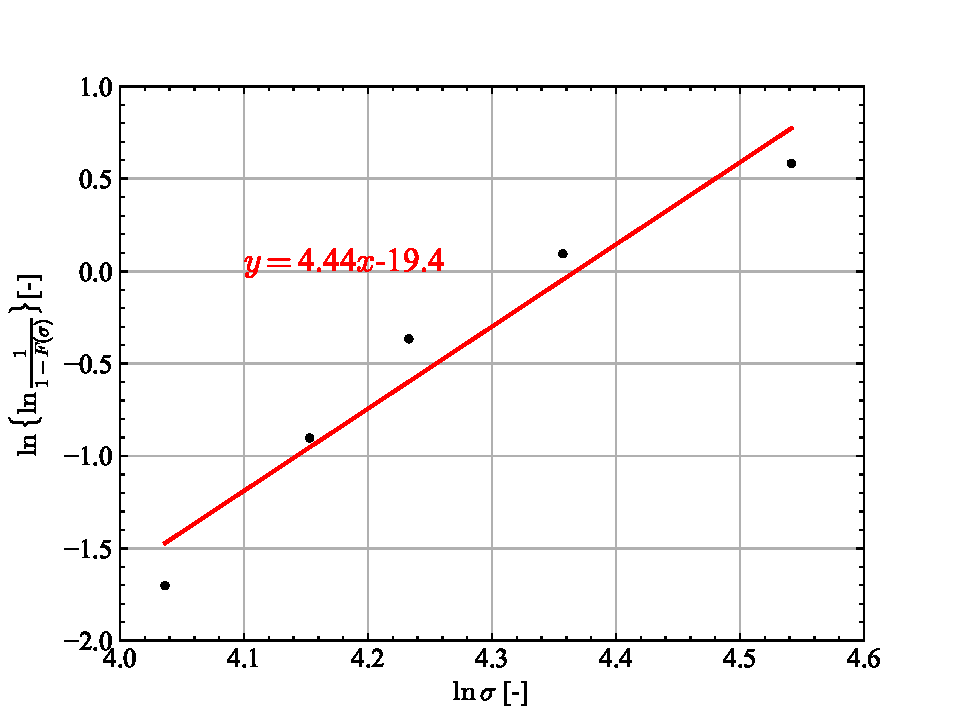
\includegraphics[width=100truemm,clip]{fig/fig_Weibull1.pdf}
    \caption{Weibull distribution for fracture stress(flawless).}
    \label{fig:ワイブル分布(傷なし)}
\end{figure}
\begin{figure}[htbp]
    \centering %中央揃え
    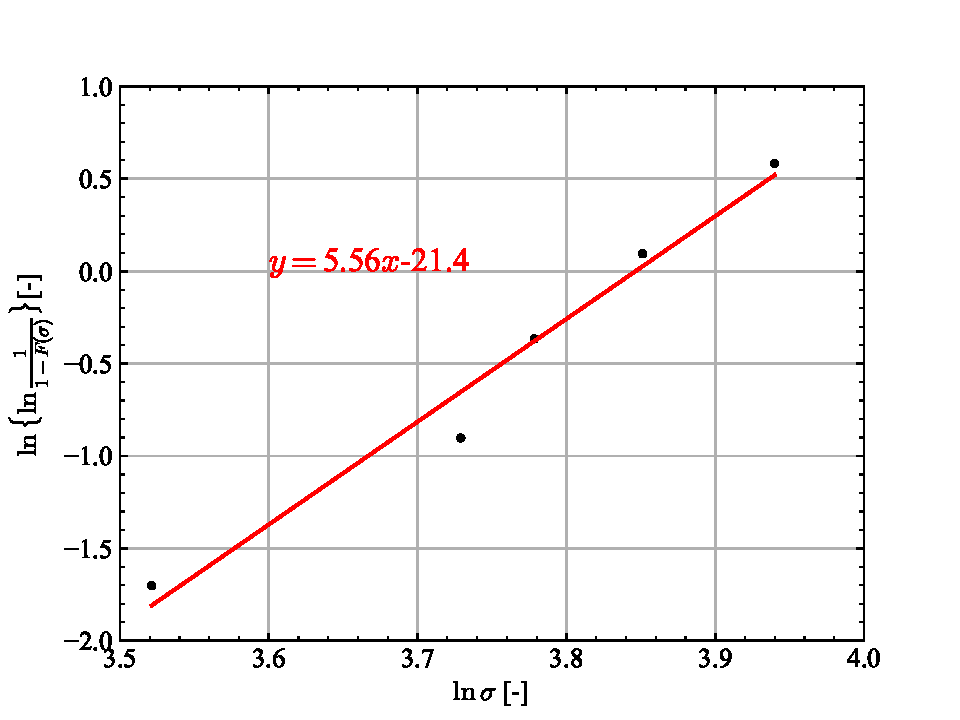
\includegraphics[width=100truemm,clip]{fig/fig_Weibull2.pdf}
    \caption{Weibull distribution for fracture stress(damaged).}
    \label{fig:ワイブル分布(傷あり)}
\end{figure}
図\ref{fig:ワイブル分布(傷なし)}の傾きと切片から,$F(\sigma)=0.5$より傷なしガラスの50\%強度は以下のように求められる.
\begin{equation}
    \sigma_{flawless} = \mathrm{exp}\lbrace \frac{ln(ln2) + 19.4}{4.44}\rbrace = 72.7[\mathrm{MPa}]
    \label{eq:傷なし50強度}
\end{equation}
同様に図\ref{fig:ワイブル分布(傷あり)}から,傷ありガラスの50\%強度は以下のように求められる.
\begin{equation}
    \sigma_{damaged} = \mathrm{exp}\lbrace \frac{ln(ln2) + 21.4}{5.56}\rbrace = 43.9[\mathrm{MPa}]
    \label{eq:傷あり50強度}
\end{equation}

\clearpage